\documentclass[convert = false, tikz]{standalone}
\usepackage[utf8]{inputenc}
\usepackage{tikz}
\usetikzlibrary{automata, positioning, arrows}
 
\usepackage{../../../../style_automata}

% arara: pdflatex
% arara: latexmk: { clean: partial }
\begin{document}
    \tikzset{
    node distance=2.5cm, % specifies the minimum distance between two nodes.
    }
    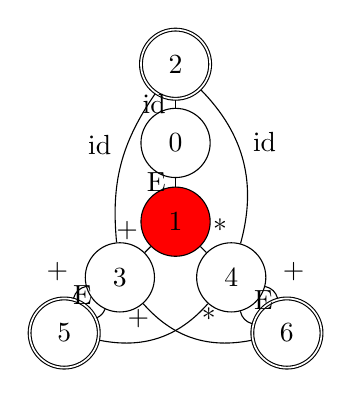
\begin{tikzpicture}
        \node[state] (0) {0};
        \node[state, fill=red, below of=0] (1) {1};
        \node[state, accepting, above of=0] (2) {2};
        \node[state, below left of=1] (3) {3};
        \node[state, below right of=1] (4) {4};
        \node[state, accepting, below left of=3] (5) {5};
        \node[state, accepting, below right of=4] (6) {6};
        \draw (0) edge[left] node{E} (1)
        (0) edge[left] node{id} (2)
        (1) edge[above left] node{+} (3)
        (1) edge[above right] node{*} (4)
        (3) edge[above left, bend left=20] node{id} (2)
        (3) edge[above left, bend left=20] node{E} (5)
        (4) edge[above right, bend right=30] node{id} (2)
        (4) edge[above right, bend right=30] node{E} (6)
        (5) edge[above left, bend left=30] node{+} (3)
        (5) edge[above left, bend right=30] node{+} (4)
        (6) edge[above right, bend right=30] node{+} (4)
        (6) edge[above right, bend left=30] node{*} (3)
        ;

    \end{tikzpicture}
\end{document}

